
\section{Optimierung des ARM}
In diesem Kapitel werden die Optimierungen am Code beschrieben, der rein auf dem ARM Cortex-A8 ausgef�hrt wird. Hierf�r werden die in \textbf{Kapitel \ref{subsec:a8}} beschriebenen Hardwareemelemte ausgenutzt.\\
In \textbf{Abschnitt \ref{subsec:armtime}} wird daher als erstes die Laufzeitmessung des gesamten Programms (Extraktion, Prozessierung und Klassifikation) erl�utert, um einen Einstiegspunkt f�r die Optimierung zu extrahieren. In den darauffolgenden Abschnitten werden daraufhin die durchgef�hrten Optimierungen beschrieben. 

\subsection{Laufzeitmessung des Gesamtprogramms}\label{subsec:armtime}
F�r die erste Laufzeitmessung des gesammten Programms (Extraktion, Prozessierung und Klassifikation) wurde dieses mit den in \textbf{Kapitel \ref{ph:neoncomp}} beschriebenen Compileroptionen zur automatischen Generierung von NEON-Code kompiliert. Die dabei resultierten Laufzeiten sind in \textbf{Abbildung \ref{fig:mclneon}} abzulesen.
%
\begin{figure}[h]
	\centering
		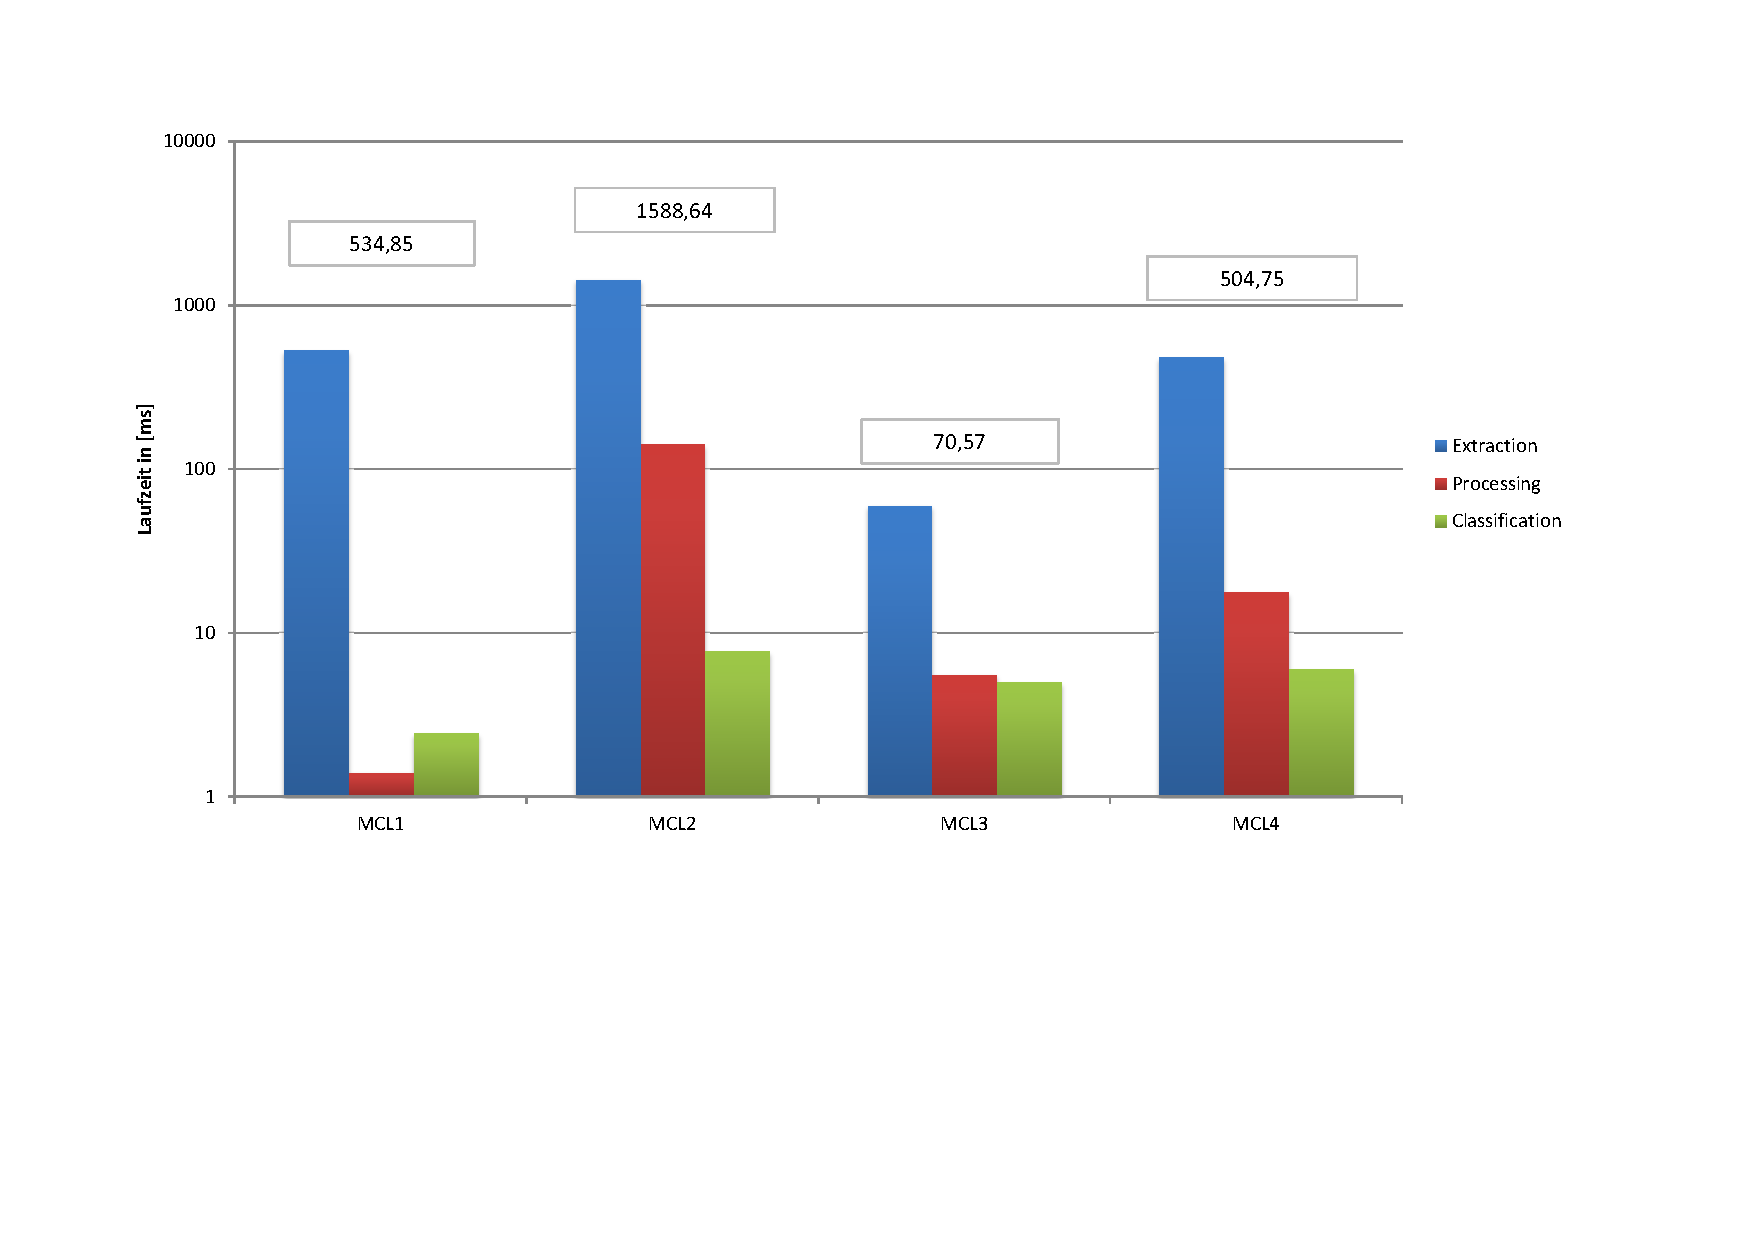
\includegraphics[width=1\textwidth]{../Pictures/mclneon.pdf}
	\caption{Laufzeiten in ms des Musikklassifikators}
	\label{fig:mclneon}
\end{figure} 
%
Wie man aus der Abbildung entnehmen kann, f�llt der gr��te Anteil an der Gesamtlaufzeit in allen vier Messungen (\textit{MCL1 - MCL4}) auf die Extraktionsphase. Es macht also Sinn diese f�r die weitere Optimierung ins Auge zu fassen.\\\\
Da die Extraktionsphase sich als am zeitintensivsten herausgestellt hat, soll diese jetzt n�her analysiert werden. Dieses und alle weiteren Messungen werden am Beispiel des in \textbf{Kapitel \ref{subsec:fset2}} beschriebenen FeatureSets durchgef�hrt, die Diagramme f�r die anderen drei FeatureSets sind f�r den interessierten Leser im Anhang zu finden, aber f�r diese sind die beschriebenen Tatsachen equivalent.\\
Wie aus \textbf{Abbildung \ref{fig:1fset2}} zu entnehmen ist, fallt der gr��te Anteil der Laufzeit der Extraktionsphase mit knapp 60\% auf die Berechnung der FFT.
%
\begin{figure}[h]
	\centering
		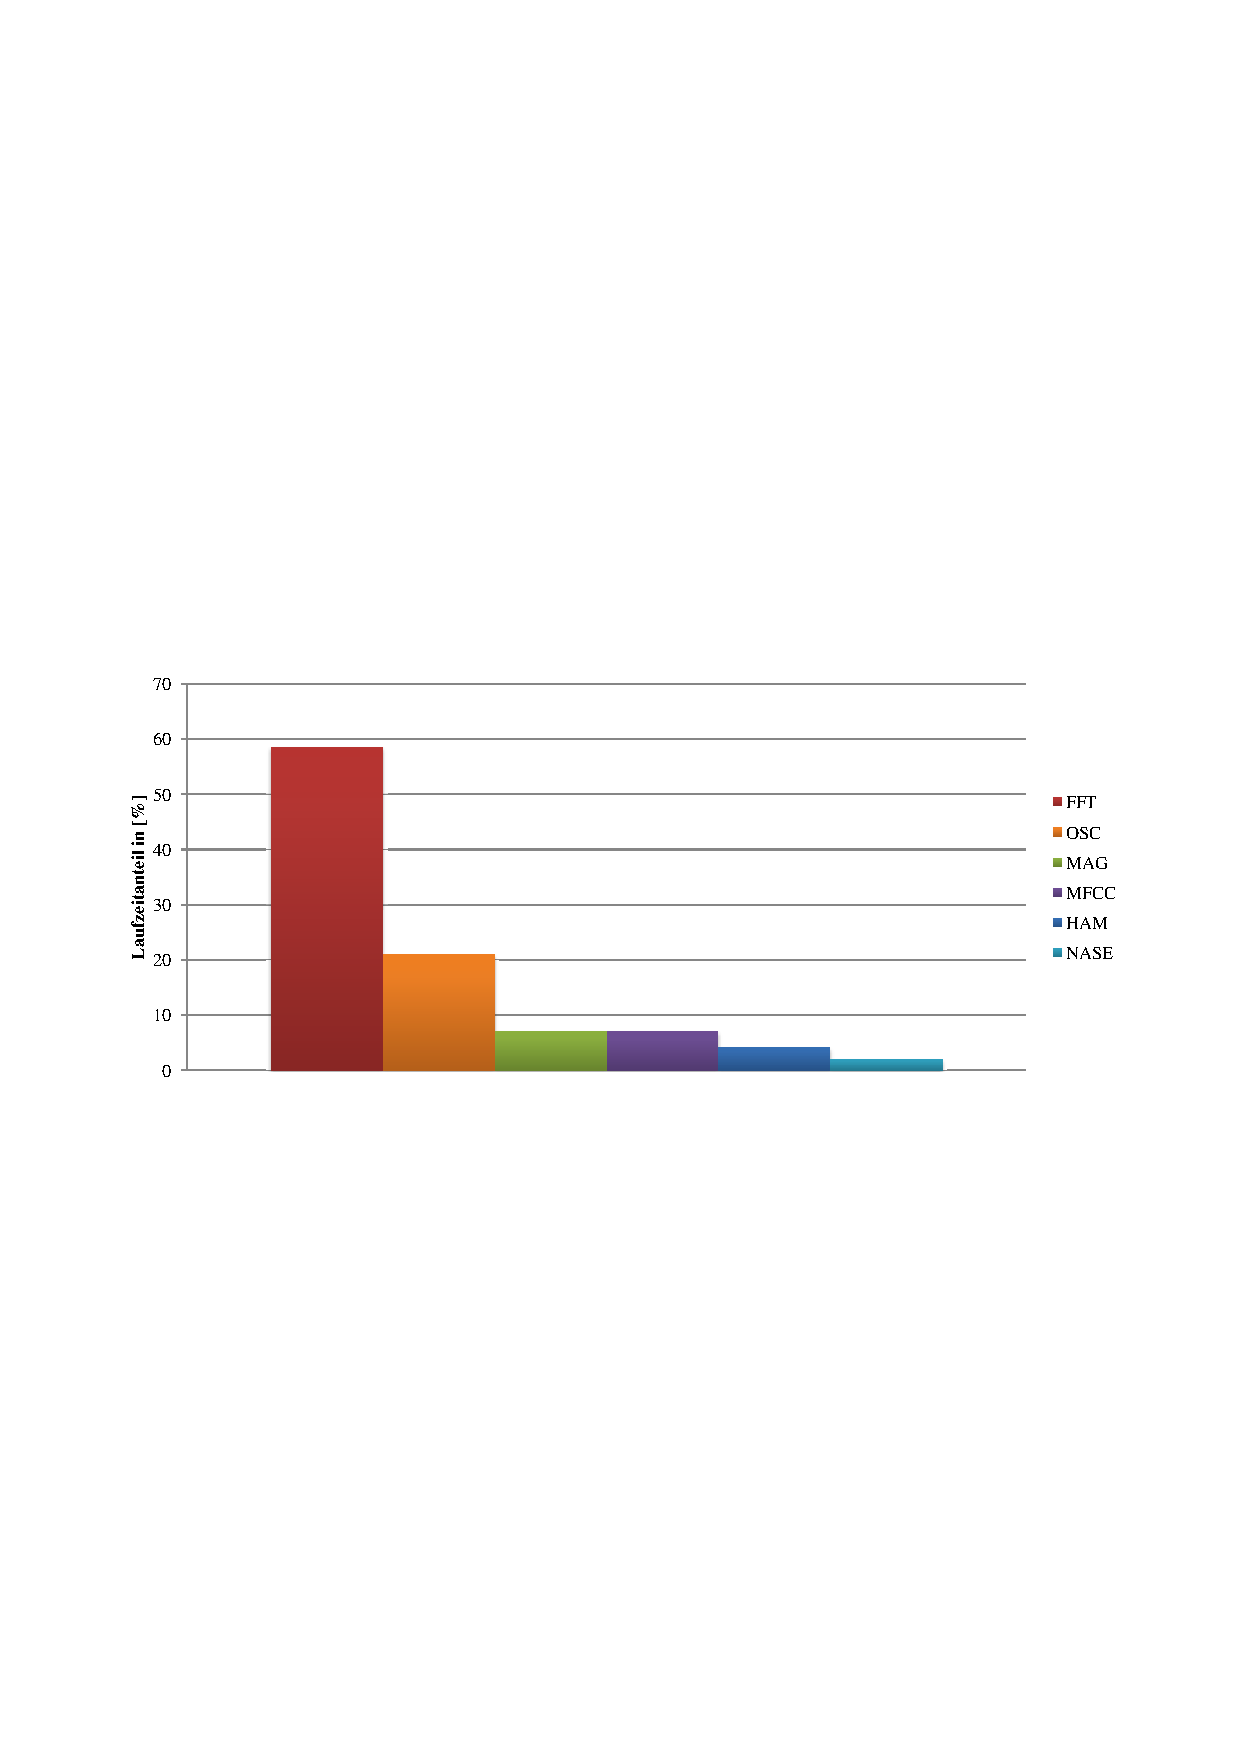
\includegraphics[width=1\textwidth]{../Pictures/1fset2.pdf}
	\caption{Detailliertere Laufzeitmessung der Extraktionsphase}
	\label{fig:1fset2}
\end{figure} 
%

\subsubsection{FFT}


\subsection{Libav als Optimierung der FFT}\label{subsec:optFFT}
\subsubsection{Laufzeitmessung}
\subsubsection{Aufbau der FFT}
\subsubsection{Einbindung}

\subsection{Optimierung der Amplitude of Spectrum}\label{subsec:optAOS}
\subsubsection{Laufzeitmessung}
\subsubsection{Codeanpassung}

\subsection{Optimierung von MFCC}

\subsection{Optimierung der Zero Crossing Rate}



 
